\documentclass[WHATMANUAL.tex]{subfiles}

\begin{document}

\section{Introduction}

The data are managed in WHAT by project, that is to say, all input and output files relative to a particular project are stored in a common folder named ``project folder''. This file management system allows to easily backup or copy the data related to a particular project since all the files are saved at the same location.

The first time WHAT is started, the software will automatically open the project ``Example'', which includes all the files necessary to easily and quickly test the different features of the software. The title of the current project is shown in the menu bar located in the upper right corner of the WHAT window. Only one project at a time can be open per instance of WHAT.

\section{Create a New Project}

The creation of a new project can be started by clicking on the \emph{New Project}~{
\includegraphics[height=2ex]{img/new_project}} button located in the menu bar (\cref{fig:WHAT_GUI}). This will open a new dialog window (\cref{fig:new_proj_win}) where information about the project can be entered such as its title, author, and location coordinates. Clicking on the button \emph{Save} will create a new project folder named after the project's title. Moreover, information related to the project are saved in a file with an extension ``.what''. It is possible to change the directory where the project is saved by clicking the folder~{
\includegraphics[height=2ex]{img/folder}} icon located next to the \emph{Save in Folder} directory path.

For example, information related to the project \emph{My New Project} by John Doe, in \cref{fig:new_proj_win}, would be saved in the file named ``My\_New\_Project.what'', in the folder named ``My New Project'', located in the directory ``\textsl{...\textbackslash{}WHAT\textbackslash{}Projects}''.

\section{Open a Project}

It is possible to open an existing project by clicking on the button \emph{Project}, which displays the name of the current project, in the upper right corner of the WHAT window. This will open a new dialog window, from which an existing project file (*.what) can be selected and opened. The current project name will then change for the name of the project that was just selected.

The path to the project folder is stored in a relative format. This means that if the location of the project folder is changed relative the executable of the software (``WHAT.exe''),  WHAT will need to be redirected to the new location of the project by repeating the procedure described in the paragraph above.

\begin{figure}[!h]
    \setlength{\fboxsep}{0pt}
    \thisfloatsetup{capbesideposition={right,bottom},
                    objectset=raggedright}
    \floatbox[\capbeside]{figure}[\FBwidth]
	{
	 \caption{Screenshot of WHAT v4.1.7-beta in Ubuntu-Linux 15.04 showing the \emph{New Project} dialog window.}
	 \label{fig:new_proj_win}
	}
	{
	 \fbox{\includegraphics[width=0.5\textwidth]{img/WHAT_Screenshot_newproject}}
	}
\end{figure}

\section{Project Folder Structure Overview}\label{subsec:folder_structure}

In addition to the project folder and the ``.what'' file that are created when saving a new project, WHAT automatically generates various files and sub-folders that are required for its execution. This file organization is briefly described below and an example is presented in \cref{fig:proFolder_organization}. The project folder contains two sub-folders named ``Meteo'' and ``Waterlvl'' and a few other files.

\paragraph{Meteo :} The sub-folder \emph{Meteo} contains three sub-folders named respectively Raw, Input and Output. The \textbf{Raw} folder is where the weather data downloaded from the CDCD are saved, for each year separately, as csv (coma-separated values) files. All the files related to a same station are saved within a common folder, named after the name of the station and its climate ID. For example, in \cref{fig:proFolder_organization}, the raw data file ``eng-daily-01011980-12311980.csv'', which contains weather data from the station ``Marieville'' for the year 1980, is saved within a folder named ``MARIEVILLE (7024627)'', where the number in parentheses is the climate ID of the station.

The folder \textbf{Input} contains the formatted weather data files produced from the raw data files. These are tsv (tab-separated values) files that are named after the name of the station, its climate ID, and the first and last year of the data record.

The folder \textbf{Output} is where the gapless weather time-series are saved in tsv files with the extension ``.out''. The files with the extension ``.log'' are tsv files that contain detailed information about the missing daily weather values that were estimated to fill the gaps in the weather datasets. The files with the extension ``.err'' contains a time-series of estimated weather values that were produced with a cross-validation re-sampling technique. These estimated values can be used to evaluate the accuracy of the method.

\paragraph{Waterlvl :} The sub-folder ``Waterlvl'' is the preferred location where the water level datasets related to a same project should be stored. These files can be  either in a Microsoft Excel spreadsheet file format (xls) or in a tab-separated values text format (tsv).

\paragraph{Other Files :} The files with an ``lst'' extension correspond to the lists of weather stations from the Canadian Daily Climate Database (CDCD) that were saved by the user from the \emph{Download Data} tab. The file ``graph layout.lst'' is a resource file, in which are stored the layout of the well hydrographs that were produced from the \emph{Hydrograph} tab. The file ``weather\_datasets\_summary.log'' is a tsv file that contains a summary of all the weather data files included in the ``Input'' folder. The file ``waterlvl\_manual\_measurements.xls'' contains all the manual water-level measurements from field visits.

\begin{figure}[!ht]
    \setlength{\fboxsep}{0pt}
    \thisfloatsetup{capbesideposition={right,bottom},
                    objectset=raggedright}
    \floatbox[\capbeside]{figure}[\FBwidth]
   	{
  	 \caption{File organization of the project folders.}
  	 \label{fig:proFolder_organization}
   	}
   	{
  	 \fbox{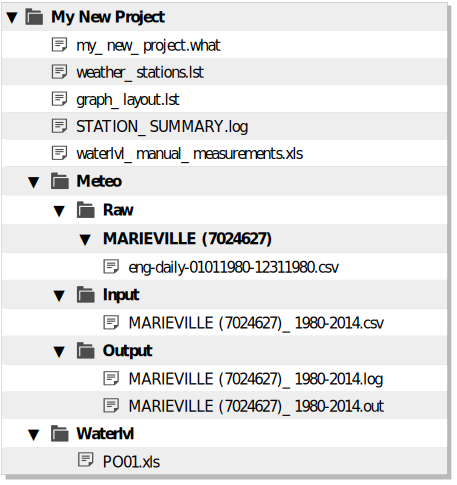
\includegraphics[width=0.5\textwidth]{img/file_and_folder_architecture}}
   	}
\end{figure}

%\FloatBarrier

\end{document}